\section{Parallelization}
\begin{enumerate}
    \item به نظر من این کد را نمی‌توان به درستی به خاطر
    \lr{data dependacy}ها
    موازی سازی کرد. اما می‌توان به نگه داشتن یک آرایه‌ی
    \lr{temp}
    و انجام ندادن به صورت
    \lr{in place}
    عملیات مشکل را حل کرد. پس کد حاصل شبیه کد زیر می‌شود:
    \codesample{codes/4-1.c}
    \item می‌توانستیم از
    \codeword{\#pragma omp critcal}
    نیز برای سینک کردن استفاده کرد ولی
    \lr{atomic}
    سریع‌تر است چرا که عملا دستورات
    \lr{atomic}
    به
    \lr{instruction}های
    \lr{CPU}
    تبدیل می‌شوند.
    \codesample{codes/4-2.c}
    \begin{figure}[H]
        \centering
        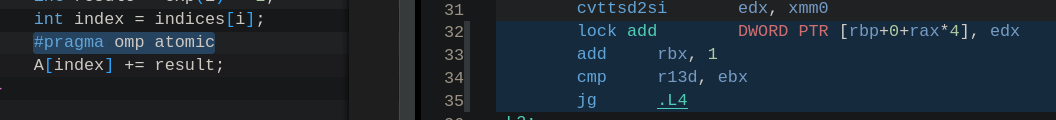
\includegraphics[scale=0.4]{pics/4-2.png}
        \caption{تبدیل شدن قسمت atomic به یک دستور با \lr{prefix lock}}
    \end{figure}
    \item از آنجا که خانه‌ی اول $B$ برابر 0 است و خانه‌ی دوم برابر ضرب خانه‌ی اول در یک عدد دیگر است،
    خانه‌ی دوم نیز برابر 0 می‌شود. با همین ترتیب کل آرایه‌ی $B$ برابر صفر می‌شود. پس می‌توان کد زیر را نوشت:
    \codesample{codes/4-3.c}
    \item یکی از کار‌هایی که می‌توان کرد این است که در یک سری از ترد‌ها در حال مقداردهی به
    $A$
    باشیم و در بقیه‌ی آنها در حال مقدار‌دهی به
    $B$. می‌توان نیز در هر
    \lr{iteration}
    نیز مثل کد سوال اول
    $A$
    را حساب کرد و سپس
    $B$
    را. برای
    $A$ به نظر من بهتر است که با توجه به
    \lr{dependacy}
    زیاد مثل قسمت اول از یک آرایه‌ی کمکی استفاده کنیم. اما برای قسمت
    $B$
    مشکلی نداریم. برای نوشتن کد
    \lr{OpenMP}
    من به مشکلی خوردم که درون یک
    \lr{section}
    نمی‌توانستم یک
    \codeword{loop}
    تعریف کنم. برای همین با کمی سرچ به
    \link{https://stackoverflow.com/a/7916905/4213397}{این}
    جواب رسیدم و با همین جواب یک کد کامل
    \lr{C}
    نوشتم. همچنین حس می‌کنم که یک
    \lr{out of bounds}
    در حساب کردن
    $A$
    داریم. این موضوع را در کد خودم درست کردم.
    \codesample{codes/4-4.c}
\end{enumerate}